

\subsection{WP1: sequence similarity sketching}
In this working package, the main objective is to sketch string similarity and output a concise binary string, such that the hamming-distance would gracefully increase as the strings become more dissimilar. Let metric $\D \colon \abcstr\times \abcstr\to R^{\ge 0}$ denote a string metric of interest, namely the edit distance. We look for a sketching function $\Sk\colon \abcstr\to\Set{0,1}^m$, such that for arbitrary strings $x,y\in \abcstr$, $\D(x,y)\approx \HD(\Sk(x),\Sk(y))$, in which $\HD$ stands for the \emph{Hamming distance} $\HD(x,y):=\#\{i\colon x_i\neq y_i\}$. One way to quantify the approximation is via \emph{distortion factor $\alpha>0$}, which informally means that the sketch-based estimate of distance is within a multiplicative $\alpha$-factor of the true distance. 
Formally, $\varphi$ has distortion $\alpha$, if there exists absolute constant $c$, such that for arbitrary strings $x,y\in S$, and distance threshold $t\in\RR^{\ge 0}$, there exists $t'\in\RR^{\ge 0}$ such that: 
\begin{equation}
\label{eq:sk_approx_factor}
\begin{cases} 
\Prob{\HD(\varphi(x),\varphi(y))> t'}\ge 1-\E^{-c \; m},& \text{if }  \D(x,y)>\alpha t\\
\Prob{\HD(\varphi(x),\varphi(y))\le t'}\ge 1-\E^{c \; m}, & \text{if } \D(x,y)\le t.
\end{cases}
\end{equation}
We can interpret \eqref{eq:sk_approx_factor} as the distortion $\alpha$ determines how much the distances can be expanded spuriously due to the sketching. 
Although the definition given here treats distortion as a constant, it is not always achievable, and $\alpha$ may depend on distance threshold $t$, sequence length $|x|,|y|$, or other parameters: $\alpha(t,|x|,|y|)$. \emph{Optimal sketching} implies that $\Sk$ achieves $\alpha=\Ocal(1)$-distortion using constant sized sketch $m=\Ocal(1)$.  


\subsubsection*{Sequence clustering}
One application for string sketching, is to cluster a large number of sequences, namely raw sequence reads, or metagenomic sequences. 
Let $S:=\Set{(s_i,g_i)}_{i\le N}$ be the list of $N$ sequences $s_i\in \abcstr$, along with their respective taxonomy code $g_i\in G$, and $S_g$ denotes the sequences belonging to $g$ $S_g:=\Set{s_i\colon g_i=g}$ The task is to estimate pairwise similarities between groups. Let us assume we interested in inter-group similarity $\Jacc_t(g,g')$ defined as number of sequences between groups $g,g'\in G$ that are $t$-close:
\[
\Jacc_t(g,g'):= \#\Set{(s_i,s_j)\in S_g\times S_{g'}\colon \D(s_i,s_j)\le t},  \qquad \norm{\Jacc_t}_1=\sum_{\Set{g,g'}\subseteq G} \Jacc_t(g,g')
\]
Definition for $J_t$ can be interpreted as soft-Jaccard similarity, as it allows for distance up to $t$ to be incorporated in similarity. If $\D(x,y)$ is the edit distance, the naive approach requires $\binom{N}{2}$ calls to the distance function $\D(x,y)$, which is prohibitive in both $N$ and length of the sequences $|x|,|y|$. Our goal to make the number of distance calls dependent on number of $t$-similar sequences, which can be substantially smaller $\norm{\Jacc_t}_1\ll N^2$. Instead, we pre-compute sketches $H:=\Set{(s_i,g_i,h_i), h_i=\Sk(s_i)}$. Due to the decay rate $\E^{-c m}$ in \eqref{eq:sk_approx_factor}, using $m:=\Ocal(\log(N))$ sized sketch suffices to have the property for for all pairs $s_i,s_j\in S$ simultaneously. Therefore, single-bit match probability $p_1$, for $t$-similar pairs, versus match probability $p_2$, for $\alpha t$-dissimilar string pairs:
\begin{equation}
\label{eq:bit_match_prob}
p_1=\min_{i\neq j}\Set{1-\frac{1}{m}\HD(h_i,h_j)\colon  \D(s_i,s_j)\le t},
p_2=\max_{i\neq j}\Set {1-\frac{1}{m}\HD(h_i,h_j) \colon \D(s_i,s_j)\ge \alpha t},
\end{equation}
A consequence of having \eqref{eq:sk_approx_factor} for all pairs is that $p_1>p_2$ with high probability. 
Using random bit-sampling, we can amplify the ratio $\frac{p_1}{p_2}$. We construct $L$ blocks, $I_1,\dots,I_L$, each of size $\ell$. To construct $I_j=\{i_1,\dots, i_\ell\}$ select each bit \iid and \uar from the set of all bits: $i_1,\dots,i_\ell\sim\Unif[m]$. Let $h_{i|I_j}$ denote the $I_j$-induced sub-sketch $h_{i|I_j}:=h_i[i_1] h_i[i_2] \dots h_i[i_\ell]$. Using the bit-collision probabilities \eqref{eq:bit_match_prob}, we can calculate the block collision probabilities.  
For all $k\in[L],i,j\in[N]$, we have:
\begin{align*}
&\Prob{h_{i|I_k}= h_{j|I_k}}\ge 1-(1-p_1^\ell)^L=:P_1 &&\D(s_i,s_j)\le t  \\
&\Prob{h_{i|I_k}= h_{j|I_k}}\le 1-(1-p_2^\ell)^L=:P_2 &&\D(s_i,s_j)\ge \alpha t 
\end{align*}
With some calculation, it can be shown that for $L=c N^\rho, \ell=\log(N)$, in which $\rho:=\frac{\log(1/p_1)}{\log(1/p_2)}<1$, we achieve $(1-P_1)\lesssim \E^{-c}$, and $P_2\lesssim 1/N^2$ (for more details see~\cite{datar2004locality}).
Based on these observations, let collision set $H(g,g')$ be defined as:
\[
H(g,g'):=\Set{(s_i,s_j)\in S_g\times S_{g'}\colon \exists k\; h_{i|I_k}= h_{j|I_k}},
\]
which we can sweep over, and decide which pairs are $t$-close 
\[
\tilde\Jacc_t(g,g'):=\# \Set{(s,s')\in H(g,g')\colon \D(s,s')\le t }.
\]
Ten, with high probability
\[
(1-\E^{-c}) \Jacc_t (g,g') \le \tilde\Jacc_t(g,g') \le \Jacc_t (g,g'), \qquad \forall g,g'\in G,
\]
requiring at most $\norm{\Jacc_{\alpha t}}_1$ distance calculations, can be substantially smaller than pairwise distance calls $\norm{\Jacc_{\alpha t}}_1\ll N^2$. 



\paragraph{Deliverables}
\begin{itemize}
\item A publication describing the method for string edit distance sketching, as well as specialized cases for gapped Hamming and shifted Hamming distance. 
\item An efficient implementation of the sketching method, plus experiments on some real-world genome datasets.
\end{itemize}

\newcommand{\AlgG}{\mathcal{A}_G}
\newcommand{\AlgL}{\mathcal{A}_L}
\newcommand{\AlgLG}{\mathcal{A}_{LG}}
\newcommand{\AlgGL}{\mathcal{A}_{GL}}

\subsection{WP 2: Sketch-based alignment}
The sketching framework which we developed on in the last working package, can be used to guide read to sequence alignment. Let us introduce some notation in order to define an alignment. Let $X,Y\subseteq \NN^{+}$ denote index sets, and $X_0:=X\cup\Set{0}, Y_0:=Y\cup\Set{0}$ append them with $0$. The precedence relation $\prec$ is defined as 
\[
(x_0,y_0)\prec(x_1,y_1) \iff ( x_0<x_1\wedge y_0<y_1) \vee (x_0<x_1 \wedge y_1=0) \vee (y_0<y_1 \wedge x_2=0)
\]
Alignment family $\Align(X,Y)$ is defined as set of all binary relations $\pi\subseteq X_0\times Y_0$, such that $\prec$ imposes a strict total order over $\pi$, and domain and co-domain of $\pi$ contain $X$ and $Y$ respectively. Alignment executions $\pi_1,\pi_2$ are defined as $\pi_1:=i_1,i_2,\dots,i_{\pi}$ and $\pi_2:=j_1,j_2,\dots,j_{|\pi|}$, where $(i_1,j_1)\prec (i_2,j_2)\prec \dots \prec (i_{|\pi|},j_{|\pi|})$ are members of $\pi$. 

For arbitrary strings $s,r\in\abcstr$, and $\pi\in\Align([|s|],[|r|])=:\Acal(s,r)$ define sequence executions as $s_{|\pi_1}:=(s[i_k])_{i_k\in \pi_1}$ and $r_{|\pi_2}:=(r[j_k])_{j_k\in \pi_2}$, where it is assumed $r[0],s[0]:=\veps$. Finally, we can define the optimal alignment:
\begin{equation}
\label{eq:optimal_alignment}
    \pi^\star(s,r) = \argmax_{\pi\in\Align(s,r)} f(s_{|\pi_1},r_{|\pi_2}).
\end{equation}
The alignment score $f(s_{|\pi_1},r_{|\pi_2})$, typically can be written as a function of the mismatch matrix $f(s_{|\pi_1},r_{|\pi_2})=\sum_{k=1}^{|\pi|} m(s[i_k],r[j_k])$, where $m:\abc_\veps^2\to\RR$ determines the penalty for gaps and mismatches. 

\subsubsection*{Guiding alignment}
It is straightforward to see that the optimal global alignment \eqref{eq:optimal_alignment}, corresponds to the edit distance if we set the $m(a,b)\gets -\1[a\neq b]$, which has a dynamic programming solution running in $\Ocal(|s||r|)$. This is considered inefficient if the query $s$ is significantly shorter than the reference $r$. If we can find the optimal starting position on the reference sequence, the complexity will be lowered to $\Ocal(|s|^2)$, since the distance cannot exceed $|s|$. 

Many alignment procedures, break the query and reference into $k$-mers as pre-processing steps in order to estimate the . For $d$-mismatches, at most $d(k-1)$ $k$-mers are touched by mismatching characters, and $|q|-(d+1)(k-1)$ are unaffected. These $k$-mers can act as anchors, where we base our alignment algorithm on. The advantage of these methods is $k$-mer exact matching can be implemented efficiently using a hash-map. The challenge is that if $k$ is too small, there will be instances of each $k$-mer, and it is not trivial how to choose the anchor, while a big $k$ risks having no untouched $k$-mer $|q|-(d+1)(k-1)\le 0$.

We propose sketch-match as opposed to $k$-mer match to be used as anchors. Let $\Set{(s_i)}_{i\le N}$ and $\Set{(r_i)}_{i\le M}$ denote $k$-mers of $s$ and $r$ respectively. Define the pair $(s_i,r_j)$ is an anchor if  $d(s_i,r_j)\le t$, which relaxes the definition to have $t$ mismatches. Therefore, we can use the same techniques outlined in the previous working package, in order to achieve sub-linear search time. 


% In this case, the time complexity grows exponentially with respect to the number of mismatches. Roughly speaking, if alignment is computed for a query sequence up to a certain point, if the next characters cannot be matched, the naive solution requires checking every possible character for alignment. In worst case, this may lead to exhausting the entire reference dataset. Therefore, many heuristics have been introduced to avoid trying visiting all search paths, similar to $A^\star$ algorithm. 

% While we described alignment and sketching over sequences, the framework can be transferred to de-Brujin graphs. 
% More specifically, suppose the reference sequence is stored on a de-Brujin Graph, and we only have the naive alignment algorithm that tries all possible paths and assigns a score to them. Moreover, the sketch values are computed in such a way that if $\D(s_q,s_i)>t$ we are guaranteed to have $\HD(h_q,h_i)>t'$. Furthermore, the sketches are stored on a subset of the vertices, with another data-structure points to next available sketch. Finally, when there are multiple outgoing edges, we can use the pointers to find the next sketch and avoid paths that point to a sketch with hamming distance above $t'$.


% For the first objective, the method is implemented and evaluated using artificially generated datasets, that mimic real genome mutations. Next, we can use a naive aligner in order to find the path with the highest alignment score. The simple aligner merely appends matching characters, and searches the space in a depth-first fashion and when there is a mismatch. The method is evaluated by replacing the query search by other sketching methods and comparing the alignment score. 
% For the second objective, we choose an aligner that relies on a heuristic to prune wrong search paths. Therefore, sketches and their distances provide the guarantee for pruning. Finally, read to reference aligner, such as MUMmer~\cite{Marcais2018MUMmer4}, may be used as baselines.



\paragraph{Deliverables}
\begin{itemize}
\item An implementation, as well as a publication, for read to reference alignment, using sensitive hashing values.
\end{itemize}


\subsection{WP 3: Syntenic region finding}
Syntenic regions are long ranges in assembled sequences, that contain multiple closely related syntenic blocks. Moreover, these blocks may be inverted, translocated, or duplicated, due to evolutionary recombination or other factors. The concrete goal of this working package to devise a locality sensitive hashing scheme, to find and align these syntenic regions. However, before we can design such a scheme, we need to formally define a syntenic region. 

Let $K$ denote the length of syntenic region, $k$ denote the syntenic block length, and $\rho_t(x,y)$ denote the similarity between $x$ and $y$ based on their edit distance, with $t$ as similarity threshold, and $\rho_t(x,y):=\1\{\ED(x,y)\le t\}$ be the hard-thresholding operator, indicating if $x,y$ are $t$-close ($1$) or not ($0$), and let $s[i:k]:=s[i,i+1,\dots,i+k-1]$ denote the $k$-mer starting at index $i$. Moreover, let $a, b\in \abc^K$ denote two syntenic regions, and $J$ designates the set of all monotonic pairings of $k$-mers:
\begin{equation}
\label{eq:def_monton_pairs}
\Align:= \Set{J\subseteq {\Ical\times \Ical}\colon \text{ if }  (i,j), (i',j')\in J,i\le i'\text{ then } j<j' }, \Ical:=\Set{1,1+k,1+2k,\dots}.
\end{equation}
The region score is formally defined as the maximum matching score between $a$ and $b$:
\begin{equation}
\label{eq:syntenic_region_score_sorted}
R(a, b,t) =  \max_{J\in \Align}
\sum_{(i,j)\in J}\rho_t(a[i:k], b[j:k]).
\end{equation}

\subsubsection*{Sketching the region score}
The region score \eqref{eq:syntenic_region_score_sorted} resembles the score function in Smith-Waterman algorithm. Let $\Sk:\abc^k\to \{0,1\}^m$ denote a sketch which for optimality ratio $c>1$, similarity threshold $t$, and collision probabilities $0\le q_2<q_1\le 1$, it satisfies:
\begin{equation}
\label{eq:ED_HD_LSH}
\begin{cases}
\ED(x,y)\le t\Rightarrow \frac{\HD(h_x,h_y)}{m}\le  1-q_1\\
\ED(x,y)\ge c t \Rightarrow \frac{\HD(h_x,h_y)}{m}\ge 1- q_2.
\end{cases}, 
\quad   x,y\in \abc^k, h_{\cdot}=\Sk(\cdot)
\end{equation}
Ideally, $q_2$ is as close to $0$ as possible, while $q_1$ is a constant larger than zero, namely $q_1>1/3$. Factor $c$ is the gap between upper and lower thresholds, which is preferably a constant close to $1$, and determines how sharp the detection is.  
Let $x_i,y_j$ denote $k$-mers $x_i=a[i:k], y_j=b[j:k]$ with sketches $h_i,g_j$ respectively, on which we define sequences
$H := h_1,h_{1+k},\dots,h_{K-k+1}$, and $G := g_{1},g_{1+k},\dots,g_{K-k+1}$.
We draw $\ell$ elements from $[m]$ uniformly at random with replacement, and repeat this process $L$ times, to construct bit-index sets $I_1,\dots,I_L$. These bit-index sets, induce sub-sketch strings $H[I_j]:=h_1[I_j],\dots,h_{K-k+1}[I_j]$, and $G[I_j]:=g_1[I_j],\dots,g_{K-k+1}[I_j]$, defined for all index sets $I_1,\dots,I_L$. 
The key idea is that the \emph{longest common subsequence (LCS)} of $H[I_j],G[I_j]\in \Set{0,1}^{\ell\star}$, is related to region score~\eqref{eq:syntenic_region_score_sorted}.

% Let $J^\star$ be the minimizer of $R(a,b,t)$, with cardinality $R=|J^\star|$, and for $i\in[R]$ define $S_i:=\Set{(x,y)\in J^\star \colon h_x[i]=g_y[i]}$. We have $\sum_{i=1}^m |S_i| \le R(1-q_1)m$. Let $|S_1|,\dots, |S_m|$ be in a non-decreasing order, $|S_i|> R(1-q_1) m/(m-i)$ leads to the contradiction $\sum_{j=i+1}^m |S_j| > R(1-q_1)m$. By union bound $\Abs{\cup_{j=1}^i S_j}\le  R(1-q_1)m i/(m-i)$, it is upper bounded by $\Abs{\cup_{j=1}^i S_j}\le R(1-q_1)m^\alpha$, if we set $i=m^\alpha,\alpha<1$. If we draw $\ell$ elements from $[m]$, with $(i/m)^\ell=m^{-1+\alpha}$ probability 

Let $\Ecal_{i,j}$ for $r\in[L]$ indicate the event $\{h_i[I_r]\neq g_j[I_r]\}$ ($1$: if it is true, $0$ otherwise), and $J^\star$ is the minimizer of $R(a,b,t)$. We have $\EE\sum_{(i,j)\in J^\star} \Ecal_{i,j} =  \Abs{J^\star}\Prob{\Ecal_{i,j}=1}$, which by property~\eqref{eq:ED_HD_LSH} is at most $R(a,b,t) {(1-q_1^\ell)}$. Therefore, by Markov's inequality we have $\Prob{\sum_{(i,j)\in J^\star} \Ecal_{i,j} \ge 4R(a,b,t) {(1-q_1^\ell)}} \le 1/4$. Let $\Ecal_{i,j}^c$ be the complement event $\Ecal_{i,j}^c:=1-\Ecal_{i,j}$, and $J^c$ be the set of $tc$-distant indices $J^c:=\Set{(i,j)\in \Ical: \ED(x_i,y_j)\ge tc}$. Using property~\eqref{eq:def_monton_pairs}, we have $\EE \sum_{(i,j)\in J^c} \Ecal_{i,j}^c \le (\frac{K}{k})^2 q_2^\ell$, and by Markov's inequality we have $\Prob{\sum_{(i,j)\in J^c} \Ecal_{i,j}^c \ge 4(\frac{K}{k})^2 q_2^\ell}\le 1/4$. Finally, combining the two by union bound, if we set $\ln(1/q_1)\lesssim\ell\lesssim \ln(1/q_2)$, and $L=\log(1/\delta)$, with failure probability $\delta$, for at least one $r\in[L]$ it holds:
\begin{equation}
    \label{eq:LCS_sandwitch}
 R(a,b,t)(1 - p_1) \le \LCS(H[I_r],G[I_r]) \le R(a,b,tc) + (\frac{K}{k})^2 p_2,
\end{equation}
in which $0<p_1,p_2<1$ are constants depending on the sketching function optimality ratio $c$, and probabilities $q_1,q_2$. Finally, since LCS similarity 2-approximates the edit distance, we can invoke the sketching function $\Sk$ on the sequences $H[I_1],\dots,H[I_L]$ and $G[I_1],\dots,G[I_L]$. Finally, if we compute componentwise Hamming distance, and report the median, the bound~\eqref{eq:LCS_sandwitch} will hold.


In the first step, we must transform the methods outlined in this package to more concrete ones, while ensuring that they approximate the corresponding biological concepts. In order to verify that the method works as expected, we must create a synthetic sequence dataset that closely follows the assumptions and definitions. Finally, the algorithm can be applied to a real dataset and compared against other syntenic aligners.  


\paragraph{Deliverables}
\begin{itemize}
\item An implementation of this approach, with application on simulated data, and two whole-genome references that are not very closely related. 
\end{itemize}


\subsection{WP 4: Multi-scale graph backbone and visualization}
% Given a de-Brujin graph $G=(V,E)$, informally, we want a ``simple`` sequence graph $T$, such that for sequences in $G$, there is a corresponding sequence in $T$ that approximates it. While the primary goal of constructing $T$ is visualization, it can also represent major variations in the set, or clean a graph constructed from raw reads. Hypothetically, a concatenation of all the reference sequences as a long simple chain contains all reference sequences with no error, yet offers no further insight about the sequences. This motivates us to put some constraint on the size of $T$. We proceed by proposing a possible formalization:


% \subsubsection*{Minimum dominating set}
% Formally, $G=(V,E)$ is the de-Brujin graph and $v\in V$ are $k$-mers, and $w(v)$ denoting the multiplicity of this $k$-mer in all our reference sequences, and for vertices $u,v\in V$, $\D(u,v)$ denotes the shortest path distance on the graph. Moreover, $\mathcal{N}(v,k)$ denotes its $k$-step neighborhood of a vertex $\mathcal{N}(v,k):=\{u\in V\colon \D(u,v)\le k\}$, which can be extended to a subset of vertices $\mathcal{N}(S,k):=\cup_{v\in S}\mathcal{N}(v,k)(v,k)$ for $S\subseteq V$. We call such a subset $(C,k)$-dominating if $\sum_{v\notin \mathcal{N}(S,k)} w(v)\le C$, and let $\mathcal{D}(C,k)$ denote all $(C,k)$-dominating sets with minimum cardinality ($|S|$ is the least possible). 
% If $S\in \mathcal{D}(C,k)$, the sequence graph induced by $v(S)$ has $|S|k$  characters,  and sum of the minimum distance of any $k$-mer in the reference sequences to $v(S)$ is bounded by $C$. 
% This optimization problem is NP-hard, as it contains a minimum dominating set problem as a special case. However, it admits approximation schemes that are efficient to compute. 

\subsubsection*{Sketch-based visualization}
The sketching scheme for syntenic region score can be readily used for visualization purposes. The first step is to visualize each genome sequence as separate paths, and if a syntenic region is found in multiple genomes, they will be joint at that location and diverge afterwards. On a lower abstraction level, the aligned syntenic blocks can be illustrated by bundling corresponding genomes, which then diverge at the location of syntenic breaks (gaps). One more detailed visualization would also indicate inverted blocks, as well as translocated and duplicated. 

This technique can be generalized to a multi-level hierarchical scheme, with each sketch recursively computed based on the lower level sketches. The main idea is to build the de-Brujin graphs on multiple levels $k_\ell=k_0 K^\ell$, and use the sketches to collapse similar $k$-mers into a single vertex. $k_0$ is the smallest word size and $K$ determines how quickly the abstraction level grows. In order to avoid the redundancy between adjacent substrings, chosen $k_\ell$-mers are at least $k_\ell/c$-apart:
$V_\ell:= \Set{s[i:k_\ell]\vert i\in \Ical_\ell}$, in which 
$I_\ell:=\Set{1,1+k_\ell/c,1+2k_\ell/c,\dots}$, and $k_0$ is divisible the absolute constant $c$. The edges at level $\ell$ are pairs of $k_\ell$-mers with a $k_\ell(1-1/c)$ overlap $E_\ell:=\Set{(s[i:k_\ell],s[i+k_\ell/c:k_\ell]): i\in I_\ell}$. Moreover, let us assume that sketching functions $\Sk\colon \abc^{k_\ell}\to  \Set{0,1}^m$ for all valid levels $\ell$, such that $\Sk(s[i:k_{\ell+1}])$ can be computed recursively using lower level sketches $\Sk(s[i:k_{\ell}])$. Furthermore, similarity edges $S_\ell$ are defined based on threshold $t$ for Hamming distance of sketches $S_\ell:=\Set{(u,v)\colon \HD(\Sk(u),\Sk(v))/m\le t}$. 
For the level $\ell$ de-Brujin graph $G_\ell:=(V_\ell,E_\ell)$, we construct backbone $T_\ell$ by copying $G_\ell$, and then contracting all similarity edges $S_\ell$ (contraction of edge $(u,v)$, removes $u$ and $v$ and creates $w$, and connects all incoming and outgoing edges to $w$). Since every $k_\ell$-mer can be uniquely mapped to a $k_{\ell+1}$-mer as its parent, vertices in $T_{\ell}$ can also be mapped to their parents in $T_{\ell+1}$. This hierarchical construction can be beneficial for characterization of genome differences, as well as multi-scale vizualization of multiple genomes. 


In terms of organizational goals, visualizing syntenic blocks and regions, with the possibility to show multiple genomes at the same time, is the only concrete objective in this package. However, the hierarchical sketching and visualization are exploratory goals, and the objective may evolve during development and experiments. 


% More formally, for the reference sequence $s$, $V(k)$ denotes the set of $k$-mers $V(k):= \Set{s[i:k]\vert i\in \Ical_k}$, starting at indices $I(k):=\Set{1,1+k/c,1+2k/c,\dots}$, in which $c$ is an absolute constant determining maximum overlap $k/c$. The edge set $E_k$ is comprised of adjacent $k$-mers $E(k):=\Set{(s[i:k],s[i+k/c:k])\vert i\in I_k}$. Let $V(k_\ell),E(k_\ell)$ denote abstraction level $\ell$ vertices and edges for scale $k_\ell=C^\ell$, in which $C$ is an absolute constant. Moreover, let $\Sk(v)\in\Set{0,1}^m$ denote a sketch function, that can be computed for all levels $v\in V(k_\ell)$, allows recursive computation of $\Sk(v)\in V(k_{\ell+1})$ based on $\Sk(v)\in V(k_\ell)$. Similarity edges $S(k_\ell)$ are defined using $t$ as similarity threshold $S(k_\ell):=\Set{(u,v)\colon \HD(\Sk(u),\Sk(v))/m\le t}$. Finally, if $G_\ell=(V(k_\ell),E(k_\ell))$ denotes the de-Brujin graph at level $\ell$, and backbone graph $T_\ell$ is defined by contraction of all similarity edges on $G_\ell$ (contraction of edge $(u,v)$, removes $u$ and $v$ and creates $w$, and redirects all incoming and outgoing edges towards $w$).


% For example, let $h_i:=\Sk(s[5i+1:10]), h_i\in\Set{0,1}^m$ denote the sketches for $10$-mers of the reference sequence $s$. Consequently, the sketch for $s[1:100]$ is recursively computed on sequence $h_0[I],\dots,h_{19}[I]$, and repeated with \iid subsampled index set $I\subseteq[m]$. The desired number of scales for visualization can be tuned by choosing the cardinality of sub-index set $|I|$, recursion factor, and overlap factor.~\footnote{recursion factor $C$ means $k$-mer sketches are computed based on $k/C$-mer sketches. Overlap factor $C$ means only for $k$-mers at indices $1,1+\floor{k/C},1+\floor{2k/C},\dots$ the sketches are computed.}.
% \subsubsection*{Random walk, leverage scores }
% Similar to before, let $V$ denote the set of all $k$-mers in our dataset. However, for any two 
% The sketching scheme outlined to find syntenic regions, can be used to add extra edges to sequence graph, indicating  
% In the same setting for $G$, plus a root node $r\in V$ that can reach all other nodes, we compute random spanning trees: starting from $r$ take out-going edges at random, in a breadth-first fashion to construct tree $T_1$, and repeat this $\ell$ times. For each node $v$, let the score  $s_i(v)$ corresponding to $T_i$ is defined the number of its descendants, the overall score is defined as the sum $s(v):=\sum_i s_i(v)$. Finally, we find the subset $S\subseteq V$, such that $G[S]$ is connected and $\sum_{v\in S} w(v)s(v)$ is maximized. The rationale behind this is that, $s(v)$ is correlated with the length of a random-walk initiated at $v$. 







\paragraph{Deliverables}
\begin{itemize}
\item A visualization algorithm and a publication, for visualization of multiple reference genomes on different abstraction scale.
\end{itemize}

% \subsection{Sketch-based optimization}









% %% Your work plan should be presented in terms of work packages, each work package representing a major piece of work. The number and nature of the work packages will depend on the topic of research and this is where the student should be guided by their supervisor. As a general guideline, a work package should describe a minimum of 3 and a maximum of 12 months of work. Each work package description should define the task and the expected outcomes. 

% %% \subsection{WP 1: My First Work Package}
% %% \paragraph{First Part of WP 1}
% %% Text goes here... lots of text.

% %% \begin{figure}[ht]
% %%   \centering
% %% 	\subfloat[]{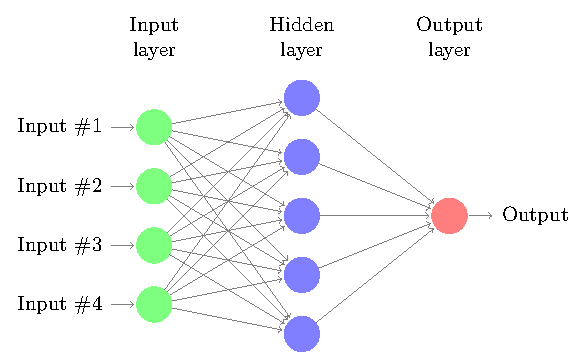
\includegraphics[width=.49\linewidth]{figures/neural-network.pdf}\label{fig:nnA}}  \hfill
% %% 	\subfloat[]{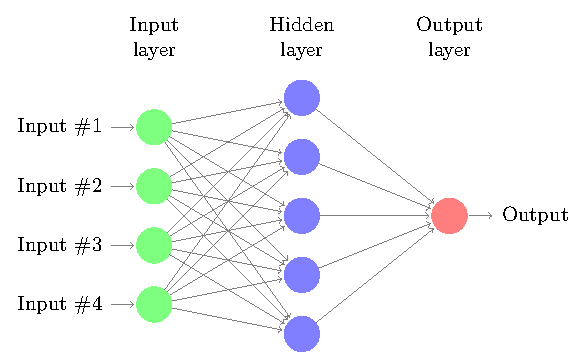
\includegraphics[width=.49\linewidth]{figures/neural-network.pdf}\label{fig:nnB}} \\
% %% \caption{\textbf{A.} A neural network. \textbf{B.} The same neural network.}
% %%   \label{fig:universes}
% %% \end{figure}

% %% \subsection{WP N: Writing the Dissertation}
% %% Writing the dissertation is planned. Things never go as planned.

% The proposed research mainly focuses on machine learning algorithms addressing the four main challenges in clinical data: heterogeneous sampling rate, irregular sampling rate, missing variables and different modalities of data.
% In the end these algorithms will be integrated into one framework which is the final goal of the proposal.
% The framework will be evaluated and compared with each algorithm alone to check if combining them will lead to improvement in performance.
% The following work packages present the outline of the main phases to tackle the research questions.

% \subsection{WP 1: Early-warning system for organ deterioration}
% In this workpackage we use ICU data collected from the ICUs of University Hospital Bern, which will be referred as Bern ICU data.
% The raw Bern ICU data come directly from the patient data management system (PDMS) of the hospital, which contains lots of artifacts caused by people misentering dates, values or variable IDs of the records.
% There are sometimes multiple records with different of the same variable for the same patients at the same time, which causes confusion because we do not know which one contains the correct measurement value.
% These artifacts need to be cleaned out before we use the data to train early-warning models.

% There exists more than 5000 variables in the Bern ICU data but not all are relevant to the organ deterioration tasks of interest, and also some are only used for short term like in clinical trails which lead to high sparseness.
% We only select variables that are most relevant to the prediction tasks as well as measured for most of the patients over most of the years in the dataset to reduce the sparseness in the final set of data that is used to train the early-warning system.
% The variable selection will be done by analyzing the statistics of the variables and with the professional knowledge from clinicians.

% After artifact cleaning and feature selection, we need to transform the data from tables to feature matrices that machine learning models can use as inputs.
% A patient will be represented by a matrix where each row corresponds to a time step and each column corresponds to a variable.
% In such matrices, there are many entries with missing values due to the heterogeneous and irregular sampling rate as well as the missing variables, which will be manually imputed.
% Labels of future organ deterioration will be computed from non-imputed data based on the definition provided by the clinicians. 
% Both non-sequential models, such as logistic regression or lightGBM, and sequential models like LSTMs will be used to predict organ deteriorations within the next 8 hours, the best one among which will be selected.
% This workpackage, where missing variables are imputed manually, establishes a baseline for the future work packages where deep learning models that can directly take non-imputed data as inputs. 

% This work is done in collaboration with Stephanie Hyland, Matthias H\"{u}ser, Martin Faltys and Tobias Merz.

% %% For the purpose of training and evaluation of the proposed algorithms and the final framework, clinical data are needed.
% %% One available clinical dataset is the ICU data collected from our collaborator, ``the University Hospital of Bern.
% %% Besides the Bern ICU dataset, two open-access ICU datasets will also be used: the MIMIC-III dataset \cite{saeed2011multiparameter} and the Philips eICU dataset \cite{mcshea2010eicu}.
% %% Since all the datasets used in the proposed research are collected from ICU, the data sampling rate usually ranges from every few minutes to once a few days.
% %% Table \ref{tbl:data} summarizes some basic information of these three datasets.
% %% \begin{table}[!ht]
% %%   \caption{Summary of the three ICU datasets we will use in the proposal.}
% %%   {\footnotesize
% %%   \begin{tabular}{p{0.225\textwidth} p{0.225\textwidth} p{0.225\textwidth} p{0.225\textwidth}}
% %%     \midrule
% %%     ~ & \textbf{MIMIC-III} & \textbf{Phillips eICU} & \textbf{University Hospital Bern} \\ \midrule
% %%     \textbf{No. of patients} & 46,520 & 139,367 & 55,476 \\ \midrule
% %%     \textbf{No. of variables} & 13,240 & 2,905 & 5,178 \\ \midrule
% %%     \textbf{No. of measurements} & $\approx 312\times10^6$ & $\approx 827\times10^6$ & $\approx 3,469\times10^6$ \\ \midrule
% %%     \textbf{Highest resolution} & $\approx 15$ minutes & $\approx 5$ minutes & $\approx 2$ minutes \\ \midrule
% %%     \textbf{Time range} & 2001 to 2012 & 2014 to 2015 & since 2005 \\ \midrule
% %%     \textbf{Demographics} & Patients at Beth Israel Deaconess Medical Centre (Boston, USA) & Patients from 459 critical care units across continental USA & Patients at University Hospital Bern (Switzerland) \\ \midrule
% %%   \end{tabular}}
% %%   \label{tbl:data}
% %% \end{table}

% %% While acquiring access to these ICU datasets is not difficult, the data do not come in a format that can be directly used by the proposed algorithms, so preprocessing the data into the desired format is an important task in this phase.
% %% Another problem is that the number of clinical variables is very large, however, a large amount of them were rarely observed.
% %% These rare variables may be observed only in some very specific patients or used in some short-term clinical trials, therefore not suitable for the general clinical problems.
% %% So one other important task in this phase is extracting commonly used and clinically important variables for general purposes.

% %% The raw ICU data directly from the patient data manangement system (PDMS) usually contain many artifacts caused by people misentering dates, values or variable ID of the observsations, or sometimes entering the same records multiple times and etc.
% %% While there are fewer artifacts in the MIMIC-III dataset and the eICU dataset because they might have been cleaned before people publish them, the Bern ICU dataset still contains quite some amount of artifacts that could significantly degrade the model peformance if ignored.
% %% Therefore, one additional task for the Bern ICU dataset is data cleaning.

% \paragraph{Deliverables}
% \begin{itemize}
% \item A set of programs that clean up the Bern ICU data, preprocess tables of ICU records and transform them into feature matrices.
% \item A medical journal paper on ICU Bern organ deterioration early-warning system.
% \end{itemize}

% \subsection{WP 2: Unsupervised representation learning from single data modality}
% This workpackage uses data from the Philips eICU dataset \cite{mcshea2010eicu}, which consists of 139367 patients and 2905 variables collected from 459 different critical care units across continental USA.
% Artifacts cleaning, feature selection, data format transformation and manual imputation also need to be applied, same as the preprocessing steps in WP 1.
% We compare non-sequential and sequential unsupervised learning techniques in terms of the representation performance in both reconstruction and prediction.
% In order to have a more objective evaluation on the generality of patients representations, we need to design a list of clinically related prediction tasks that covers a wide range of clinical concepts.
% The dynamic diagnosis and treatment records satisfy such requirement. 

% The non-sequential unsupervised representation learning techniques we use are PCA and vanilla autoencoder, and the sequential ones are variations of sequence-to-sequence model.
% Sequence-to-sequence models can be used as an autoencoder, i.e. the decoder reconstructs the input sequences; but it can also be used as a forecaster, which predict the future sequence of the current input sequences.
% Between a forecaster and an autoencoder with the same number of parameters, a forecaster has the advantage of ``seeing'' some future information than just the history during training, hence representations learned by the forecasters should be more predictive of the future events.
% Attention mechanism will also be added to the sequence-to-sequence forecaster under the intuition that feature values at each future time point may have higher relevance to only a local region of the input sequence. 

% \paragraph{Deliverables}
% \begin{itemize}
% \item A conference paper that benchmarks the unsupervised representation learning methods on medical time series.
% \end{itemize}

% \subsection{WP 3: Learning from multirate irregular time series}
% The data used for this workpackage are the commonly observed numerical variables.
% Missing variables will be imputed with global mean or expert-defined normal values.
% The data will be resampled to be on a fixed-interval time grid to remove the irregularity.
% Sampling rate of the data will be made sure to be in these three range: every few minutes, every few hours and once a day.
% In the baseline method, the time series will be imputed with forward-filling.

% The clinical problem of interest is learning representations that can be used to predict diagnosis/treatments in the future. 
% Different representation learning methods in a either supervised or unsupervised fashion will be studied in order to establish the best baseline.
% In the best representation learning model, the parts that takes the time series as inputs will be replaced with Phased LSTM, multi-rate LSTM and the proposed algorithm respectively, so that it will be able to take non-imputed multi-rate time series as inputs, and the former two will be the state-of-the-art baseline for the last one to compare against.
% The performance of the proposed method and the baselines will be evaluated on the representation performance in the diagnosis/treatment prediction tasks.

% Two naive baselines will be used in dealing with irregularity, in both of which standard LSTMs will be used, but one will ignore the irregularity by ``pretending'' that two consecutive observations always have a fixed time interval and the other uses data resampled to a fixed-interval time grid.
% Besides the two naive baselines, the proposed method will also be compared with T-LSTMs as the state-of-the-art baseline.
% \paragraph{Deliverables}
% \begin{itemize}
% \item Design, definition and implementation of the proposed algorithm.
% \item Two conference papers will be written presenting the proposed algorithms.
% \end{itemize}

% \subsection{WP 4: Learning from time series with missing variables}
% The data used in this work package will still be similar to those in WP 2, with the only difference that the missing variables will not be imputed.
% Since the research at this phase focuses on dealing with missing variables, the time-series will also be forward-imputed to remove the multirate aspect.
% The clinical problem is diagnosis prediction or medicine recommendation.

% Standard LSTMs will be applied to the data with missing variable values imputed by the statistical global mean or the expert-defined normal values.
% Methods and metrics to measure the similarity between time series will be designed so the temporal components can also be incorporated into the CF framework for the clinical problem.
% \paragraph{Deliverables}
% \begin{itemize}
% \item Design of the similarity measurement method and metric for time series.
% \item A conference paper will be written presenting CF over clinical time series with missing variables.
% \end{itemize}

% \subsection{WP 5: Representation learning from heterogeneous data modalities}
% In this work package, we will implement a joint model that combines Med2Vec \cite{choi2016multi} and the representation learning algorithm for numerical clinical variables developed in WP 2.
% Representations learned from the joint model will be compared with the Med2Vec representations and WP-2 representations in terms of their prediction performance in the organ deterioration early-warning task mentioned in WP 1. 

% %% In this work package, the methods from WP 2, 3, 4 will be integrated into a united model that uses only numerical time-series data as input.
% %% Time series of texts will be encoded into time series of word embeddings using GloVe, and time series of medical codes will be encoded by Med2Vec.
% %% The time series of embeddings will be treated the same as the numerical time series and be input to the aforementioned combined time-series model.
% %% The entire framework will be compared with the combined model that only uses numerical clinical variables to check if incorporating more data will improve the performance.
% \paragraph{Deliverables}
% \begin{itemize}
% \item A represenation model that take both numerical clinical variables and medical codes as inputs.
% \end{itemize}

% \subsection{WP 6: Writing the Dissertation}
% Writing dissertation to summarize all the previous works.
